\documentclass[tikz,border=8pt]{standalone}
\usepackage{amsmath,amssymb}
\usetikzlibrary{arrows.meta,calc,decorations.markings,decorations.pathmorphing,patterns,shapes.geometric,positioning}

\begin{document}
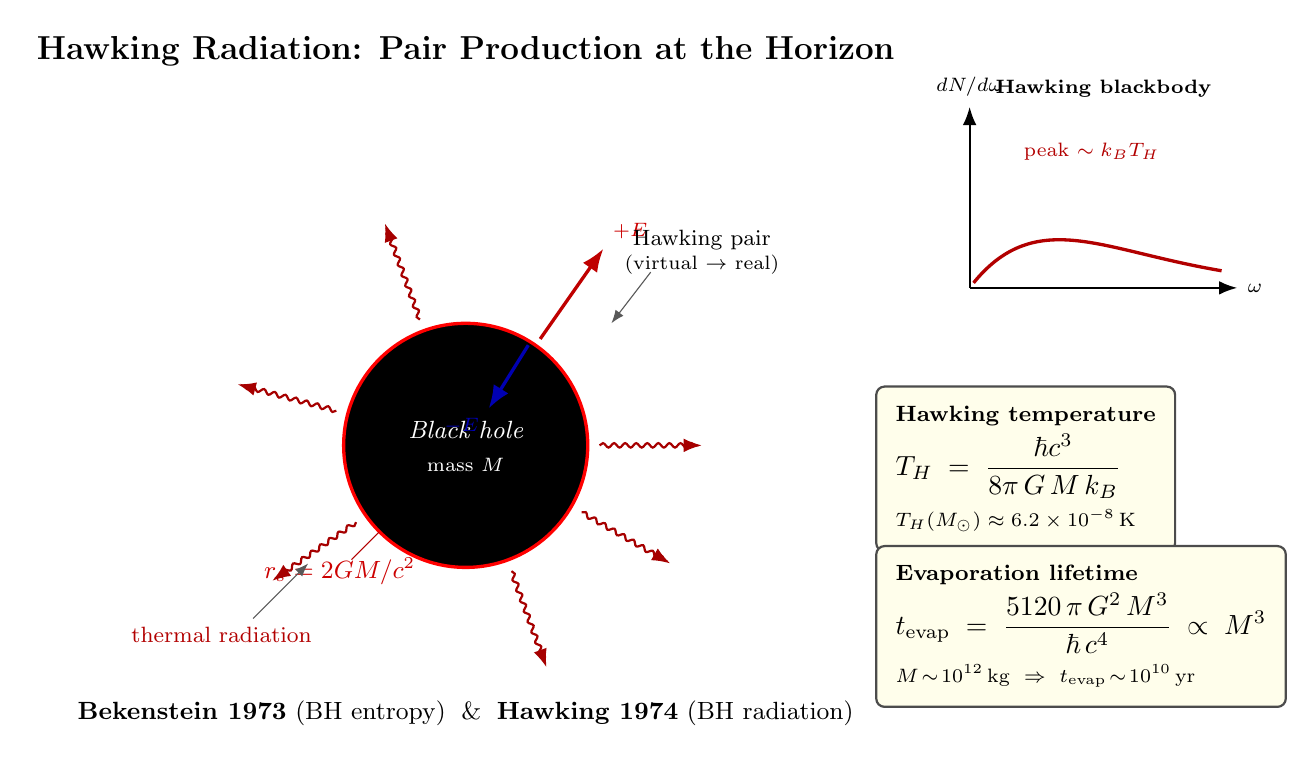
\begin{tikzpicture}[>=Latex,
  outparticle/.style={->, very thick, red!75!black},
  inparticle/.style={->, very thick, blue!70!black},
  thermalray/.style={->, thick, red!65!black, decorate,
                     decoration={snake, amplitude=0.8pt, segment length=4pt, post length=2pt}},
  formulabox/.style={rectangle, draw=black!70, thick, rounded corners=3pt,
                     fill=yellow!8, inner sep=7pt, align=left}]

  % --- Title -----------------------------------------------------------------
  \node[font=\large\bfseries, align=center] at (0, 5.0) {%
    Hawking Radiation: Pair Production at the Horizon};

  % --- Black hole disk -------------------------------------------------------
  \fill[black] (0,0) circle (1.55);

  % --- Event horizon (red) ---------------------------------------------------
  \draw[red, very thick] (0,0) circle (1.55);

  % horizon label
  \node[red!80!black, font=\small] at (-1.6, -1.6) {$r_s = 2GM/c^2$};
  \draw[red!70!black, thin] (-1.45,-1.45) -- (-1.1,-1.1);

  % "Black hole" label inside
  \node[white, font=\small\itshape] at (0, 0.2) {Black hole};
  \node[white, font=\scriptsize] at (0, -0.25) {mass $M$};

  % --- Pair production at the horizon (upper-right, ~45 deg) ------------------
  % the pair appears just outside the horizon
  \coordinate (pairout) at ($(0,0)+({1.65*cos(55)},{1.65*sin(55)})$);
  \coordinate (pairin)  at ($(0,0)+({1.50*cos(58)},{1.50*sin(58)})$);

  % outgoing positive-energy particle (red)
  \draw[outparticle] (pairout) -- ($(pairout)+({1.4*cos(55)},{1.4*sin(55)})$);
  \node[red!80!black, font=\scriptsize, anchor=south west] at ($(pairout)+({1.4*cos(55)},{1.4*sin(55)})$) {$+E$};

  % infalling negative-energy partner (blue)
  \draw[inparticle] (pairin) -- ($(0,0)+({0.55*cos(58)},{0.55*sin(58)})$);
  \node[blue!70!black, font=\scriptsize, anchor=north east] at ($(0,0)+({0.55*cos(58)},{0.55*sin(58)})$) {$-E$};

  % "Hawking pair" label
  \node[font=\footnotesize, align=center] at (3.0, 2.45) {Hawking pair\\[-1pt]\scriptsize (virtual $\to$ real)};
  \draw[->, thin, gray!70!black] (2.35, 2.20) -- (1.85, 1.55);

  % --- Outer thermal radiation arrows (multiple wavy arrows around BH) -------
  \foreach \angle in {0, 110, 165, 215, 290, 330}{%
    \draw[thermalray]
      ($(0,0)+({1.7*cos(\angle)},{1.7*sin(\angle)})$) --
      ($(0,0)+({3.0*cos(\angle)},{3.0*sin(\angle)})$);
  }

  % "thermal" label
  \node[font=\footnotesize, red!70!black] at (-3.1, -2.4) {thermal radiation};
  \draw[->, thin, gray!70!black] (-2.7, -2.2) -- (-2.0, -1.5);

  % --- Right-side mini blackbody spectrum plot --------------------------------
  \begin{scope}[xshift=6.4cm, yshift=2.0cm]
    % axes
    \draw[->, thick] (0,0) -- (3.4, 0) node[anchor=west, font=\scriptsize] {$\omega$};
    \draw[->, thick] (0,0) -- (0, 2.3) node[anchor=south, font=\scriptsize] {$dN/d\omega$};

    % Hawking blackbody-like curve: omega^2/(e^omega - 1)
    \draw[red!70!black, very thick, smooth, samples=80, domain=0.05:3.2]
      plot (\x, {1.85 * (\x*\x) / (exp(1.4*\x) - 1)});

    % label peak
    \node[font=\scriptsize, red!70!black, anchor=south] at (1.55, 1.50) {peak $\sim k_B T_H$};

    % title
    \node[font=\scriptsize\bfseries, anchor=south] at (1.7, 2.30) {Hawking blackbody};
  \end{scope}

  % --- Formula box: T_H ------------------------------------------------------
  \node[formulabox, anchor=west] at (5.2, -0.3) {%
    \footnotesize\textbf{Hawking temperature}\\[2pt]
    $\displaystyle T_H \;=\; \frac{\hbar c^{3}}{8\pi\,G\,M\,k_B}$\\[3pt]
    \scriptsize $T_H(M_\odot) \approx 6.2\times 10^{-8}\,\mathrm{K}$
  };

  % --- Formula box: t_evap ---------------------------------------------------
  \node[formulabox, anchor=west] at (5.2, -2.3) {%
    \footnotesize\textbf{Evaporation lifetime}\\[2pt]
    $\displaystyle t_{\rm evap} \;=\; \frac{5120\,\pi\,G^{2}\,M^{3}}{\hbar\,c^{4}} \;\propto\; M^{3}$\\[3pt]
    \scriptsize $M\!\sim\!10^{12}\,\mathrm{kg}\ \Rightarrow\ t_{\rm evap}\!\sim\!10^{10}\,\mathrm{yr}$
  };

  % --- Footer ----------------------------------------------------------------
  \node[font=\small, align=center] at (0, -3.4) {%
    \textbf{Bekenstein 1973} (BH entropy) $\;\&\;$
    \textbf{Hawking 1974} (BH radiation)};

\end{tikzpicture}
\end{document}
